79. $\cfrac{x^2+y-2}{x+3}=0\Leftrightarrow\begin{cases}y=2-x^2,\\ x\neq-3.\end{cases}$
$$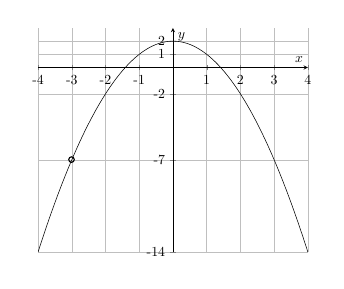
\begin{tikzpicture}[scale=0.5]
\begin{axis}[
    axis lines = middle,
    grid=major,
    legend pos={south west},
    xlabel = {$x$},
    ylabel = {$y$},
    ymin=-14,
    ymax=3,
    xtick={-3, -4, -1, 1, 4,3, 6,-2,2,8},
    xticklabels={-3, -4, -1, 1, 4,3, 6,-2,2,8},
    ytick={-14,-7,-2,1,2},
    yticklabels={-14,-7,-2,1,2}            ]
	\addplot[domain=-4:4, samples=100, color=black] {2-x*x};
%\addplot[domain=-3.1:2.5, samples=100, color=red] {70*abs(1-2*abs(abs(x)-2))-10*x^2+10*x-70};
	%\addlegendentry{$\text{Рис. 1}$};
\end{axis}
\draw (0.85,2.35) circle (2pt);
\end{tikzpicture}$$
Равноудалены от осей координат те точки, у которых $|y|=|x|,$ то есть $|2-x^2|=|x|\Leftrightarrow$\\$\left[\begin{array}{l} 2-x^2=x,\\ 2-x^2=-x.\end{array}\right.
\Leftrightarrow\left[\begin{array}{l} x^2+x-2=0,\\ x^2-x-2=0.\end{array}\right.\Leftrightarrow\left[\begin{array}{l} (x+2)(x-1)=0,\\ (x-2)(x+1)=0.\end{array}\right.$ Значит, это точки $(-2;-2),(2;-2),$\\$(-1;1),(1;1).$\\
